
%%%%%%%%%%%%%%%%%%%% file CSMC_MUME_LaTeX_Template.tex %%%%%%%%%%%%%%%%%%%%%
%
% This is the LaTeX source for the instructions to authors using
% the LaTeX document class 'llncs.cls' for contributions to
% the Journal of Creative Music Systems.
% Copyright: http://www.springer.com/lncs       Springer Heidelberg 2006/05/04
%
% It may be used as a template for your own input - copy it
% to a new file with a new name and use it as the basis
% for your article.
%
% NB: the document class 'llncs' has its own and detailed documentation, see
% ftp://ftp.springer.de/data/pubftp/pub/tex/latex/llncs/latex2e/llncsdoc.pdf
%
%%%%%%%%%%%%%%%%%%%%%%%%%%%%%%%%%%%%%%%%%%%%%%%%%%%%%%%%%%%%%%%%%%%

\documentclass[runningheads,a4paper]{llncs}

\usepackage{amssymb}
\setcounter{tocdepth}{3}
\usepackage{graphicx}
\usepackage{url}
\usepackage{apacite}
%added 
\usepackage[inline]{enumitem}    
\usepackage{subcaption}
\usepackage{caption}
\usepackage{threeparttable} %annotations for table
\usepackage{csquotes}
\usepackage{appendix}

\newcommand{\keywords}[1]{\par\addvspace\baselineskip
\noindent\keywordname\enspace\ignorespaces#1}

\pagestyle{headings}

\begin{document}

\mainmatter  

\title{Percussive Sound Generation with Virtual Listeners and Modular Synthesizers}

% a short form should be given in case it is too long for the running head
\titlerunning{Virtual Percussive Sound Generation}

% the name(s) of the author(s) follow(s) next
\author{Amir Salimi \and Abram Hindle}

\authorrunning{Amir Salimi and Abram Hindle }

% the affiliations are given next; don't give your e-mail address
% unless you accept that it will be published
\institute{Department of Computing Science\\ University of Alberta \\ \email{asalimi@ualberta.ca\\ }}

% intro, 1 page
% background and methodology 2 pages
% implementation 
% results 2.5
\maketitle

\begin{abstract}
Can we generate drum synthesizers automatically?
We present an approach for the automatic generation of synthesizer programs for one-shot percussive sounds. 
Recent advancements in digital synthesis, heuristic search, and neural networks can be utilized for sound generation. 
Yet the need for data, the problem of open set recognition, and high computational costs persist as barriers towards the expansion of sound libraries using these techniques. 
We generate quick, scalable, percussion synthesizers using classical signal processing. 
We train drum classifiers to find and classify synthesizer programs that mimic percussive sounds. 
We use features from Fourier transformations and autoencoder embeddings to train machine learning classifiers.
Manual listening tests of the generated sounds demonstrates the system can successfully generate drum synthesizers and categorize drum sounds.
To facilitate future research, we share our curated dataset of free percussive sounds.
\keywords{Automatic Synthesizer design. Machine Listening. Sound Analysis. Novelty and Originality}
\end{abstract}


\section{Introduction} 
Digital recordings of novel, one-shot\footnote{A single hit on the drum that captures its capabilities} drum sounds are commonly used in  electronic music compositions. Yet unique drum sounds can be difficult or expensive to find. By relying on recordings of \textit{real life} drum sounds, artists are limited by what instruments exist in the real world and whether or not high-quality, one-shot recordings can be accessed. We believe automatic programming of virtual synthesizers for the creation of novel drum sounds can alleviate these material limitations. To this end, we implement a programmable virtual synthesizer of audio, which we call the \emph{virtual synthesizer}. We also implement machine learning classifiers for automatic separation of percussive sounds from non-percussive sounds. To effectively train the classifiers with small datasets, we simplify the representation of audio data by experimenting with fast Fourier transform (FFT) features and autoencoder embeddings. We call our system of feature extraction and classification of sounds the \emph{virtual ear}. To create a dataset of synthetic drums, the virtual synthesizer produces random programs and generates the corresponding audio. This audio is then categorized by the virtual ear. We save not just the desirable sounds, but also the programs which generated these sounds. These programs can be modified and experimented on by sound designers, or used for an improved search algorithm in future works. We build generative systems using different implementations of the virtual ear, and conduct manual hearing tests of the generated sounds. Our results are promising as the majority of sounds generated from our systems are deemed percussive by human listeners. However, we cannot quantify the novelty of these sounds. 

 \begin{figure}[t]
    \begin{center}
    % \textbf{Generative System}
    \makebox[\textwidth]{
    \fbox{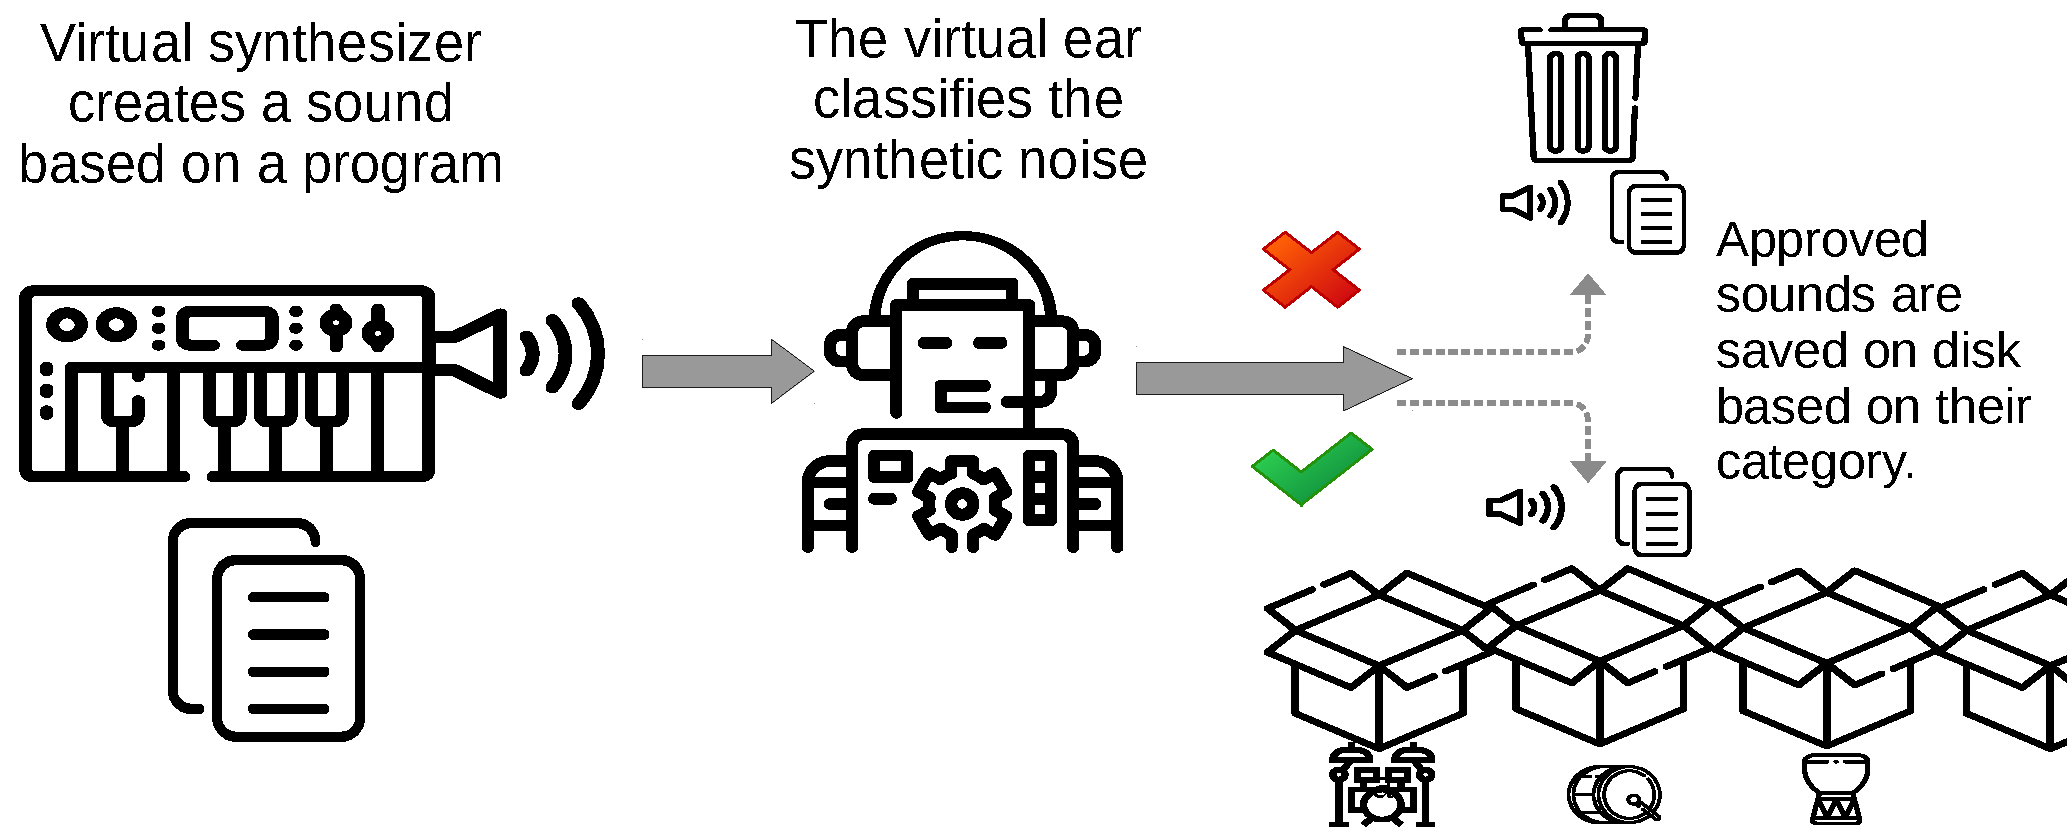
\includegraphics[width=1\linewidth]{images/pipeline.pdf}}}
    \end{center}
    \caption{A blueprint of our system which allows each component to be implemented in a number of ways. Our implementations of this pipeline allow for easy parallelization when needed. This implementation also allows for easy integration of heuristic search for future works. 
    }
\label{fig:pipeline_outline}
\end{figure}

\section{Related Works}
Numerous deep neural network models have been proposed for the purpose of signal generation in recent years. WaveGans and WaveNet have been subject to significant improvements and experiments since their proposal~\cite{nsynth2017,yamamoto2020parallel,oord2017parallel}. Particularly relevant works are the utilization of variational autoencoders (VAE's) for generation of percussive samples~\cite{aouameur2019neural} and generation of percussive sounds by decoding a small set of latent features~\cite{ramires2020neural}. Automatic programming of virtual synthesizers has long been a topic of interest. In early 2000s, Interactive Genetic Algorithms (IGA's) were utilized for the generation of new sounds with various sound-engines~\cite{johnson1999exploring,dahlstedt2001creating}. More recent work by Yee-King et al.~\cite{yee2018automatic} used Long short-Term Memory (LSTM) models and genetic algorithms to find the exact parameters used to create a group of sounds. The sounds approximated were made by the same virtual synthesizer and not with an external source, making the eventual replication certain even with random search. Yet another recent work by Esling et al. used a large dataset of over 10,000 presets for a commercial VST synthesizer to learn a latent parameter space which can be sampled for creation of new audio~\cite{esling2019universal}. Here, we work towards the approximation of percussive sounds with no previous knowledge about the sonic capabilities of a virtual synthesizer.

\section{Virtual Synthesizer Design}
\begin{table}[htbp]
\centering
\resizebox{\columnwidth}{!}{\begin{tabular}{ |p{4cm}|p{4cm}|p{4cm}| } 
\hline
Parameters & Value Range & notes and constraints\\
\hline \hline
Attack & 0-3 & A-D-S-R values relative\\
Decay & 0-3 & relative to A-S-R\\
Sustain & 0-3 & relative to A-D-R\\
Release & 0-3 & relative to A-D-S\\
OSC type & sine,square,saw & -\\
IsNoise & boolean & generate noise using \newline cloud of waveform\\
Length & 0-1 second & - \\
StartTime & 0-1 second & Length+Start$<$1\\
Amplitude & 0.1-1 & 1 = max amplitude\\
Pitches(notes) & list of pitches &  range of C0(16.35hz) to B9 \\
HP filter Cuttoff & 0-20000hz & -\\
LP filter Cuttoff & 20000-HP & never lower than HP cutoff\\
Filter Order & 4,8,16 & butterworth filter order \\
\hline
\end{tabular}}
\caption{Synthesizer submodule parameters. Despite the simplicity of the parameters and our efforts at constraining the ranges, the number of parameters that can be randomly chosen for each submodule is over $10^{15}$. Each synthesizer can contain any number of submodules}
\label{table:submodule_params}
\end{table}
Digital sound is a series of discrete values. \textit{Digital synthesis} of audio is the process of creating these values. Here, we do not employ probabilistic models for the synthesizer component. Our decision is based on the following factors:
\begin{itemize}
    \item \textit{Novelty and Creativity}: Given large sets of examples, generative models such as VAEs and GANS have proven capable of generating samples similar to the exemplars. In this work, we are not aiming for perfect imitations. We seek to create \emph{novel sounds} by via artificial, exploratory creativity. Boden defines this concept as an emergent property of generative work within confined rule sets~\cite{boden2009computer}. Ultimately, we wish to work within the limitations of any tractable sound source to create its approximations of a given sound category. Within the music realm, a prominent instance of exploratory creativity is the persistent aesthetics of 8-bit soundtracks, remaining popular long after the original constraints are lifted~\cite{collins2007loop}.
    \item \textit{Interpretability}: Neural networks are often described as black boxes~\cite{basheer2000artificial}. Their highly recursive structure makes modern explanation methods such as saliency maps unreliable~\cite{rudin2019stop}.  
    \item \textit{Speed of Rendering at high sampling rates}: Despite the utilization of powerful GPUs, the standard sampling rate in most audio generation work utilizing neural networks is under 24 khz ~\cite{yamamoto2020parallel,oord2017parallel,aouameur2019neural,ramires2020neural}. However, a significant number of untrained human ears can detect a change in quality of audio between sampling rates of 192 khz and the industry standard of 44.1 khz \cite{reiss2016meta}. At our fixed sampling rate of 48 khz, synthesizers with stack sizes of 8 can create and save 1 sounds to hard-disk with an average rendering time of 50 milliseconds\footnote{Using a single process on a Macbook Air 2012 and Ubuntu 18.04}. 
    \item \textit{Flexibility and Scaling}: Probabilistic audio generation is often done sequentially. For example, state of the art, parallel wave generation with GANs requires a fixed amount for rendering time for each time-step~\cite{yamamoto2020parallel}. Our virtual synthesizer produces audio by solving a linear system of equations. The added footprint of increasing the length of rendered sounds or higher sampling rates is relatively minuscule.  
\end{itemize}

%  Evaluation of a periodic function such as sine or cosine is the simplest form of software audio generation~\cite{mitchell2009basicsynthChap5}. This generative system is called an \textit{oscillator}. With careful programming, DSP techniques can be used to replicate almost any sound~\cite{jenkins2019analog}. Synthesizers we build using these functions are tractable and explainable: the output is determined by the input and reproducible. This makes the evaluation of a set of inputs (or parameters) to our synthesizers relatively simple.
 
 \begin{figure}[t]
    \begin{center}
    % \textbf{Synthesizer SubModule }
    \makebox[\textwidth]{
    \fbox{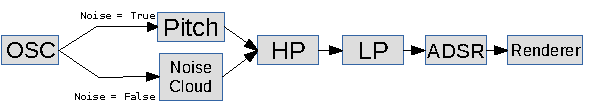
\includegraphics[width=1\linewidth]{templates_aimusic2020/images/synthesizer_block.pdf}}}
    \end{center}
    \caption{High level representation of pre-rendering steps for each submodule. Each Synthesizer contains 1 or more these submodules. The output of a synthesizer is the normalized addition of all its submodule outputs. Each synthesizer program determines the number of these submodules and their parameters. 
    }
\label{fig:pipeline_outline}
\end{figure}


We rely on a set of classical DSP methods to build our synthesizer, which allows for quick, offline, and parallel generation of audio signals without the usage of GPUs. We made extensive use of Pippi\footnote{https://github.com/luvsound/pippi} and SciPy~\cite{jones2001scipy} libraries. Our virtual synthesizer contains a set of one or more submodules. Each submodule is a self-contained noise making unit. Submodules have identical sets of parameters, but widely different outputs can be achieved depending on the values assigned. The set of parameters available to each submodule is highlighted in Table~\ref{table:submodule_params}. The sonic output of the virtual synthesizer is the normalized addition of the sonic output of its submodules. Our implementation of a synthesizer can have any number of submodules. The parameters that dictate the output signal of each submodule as well as the range of values each parameter can take are shown in table~\ref{table:submodule_params}. We call the number of submodules in each virtual synthesizer the \textit{stack size}. We call the sets of parameter values that characterize a synthesizer's submodules a \textit{program} (analogous to a preset for a VST).   

\section{Virtual Ear}
The task assigned to the virtual ear is the rare acceptance of drum-like sounds and the inevitable rejection of most \enquote{noise} outputs from the virtual synthesizer. Our goal is not realism; We want the virtual ear to accept novel and unusual drum sounds. The virtual ear makes two critical decisions: 
\emph{
\begin{quote}
\text{Decision.1 Could the sound be used as a drum?}\label{Decision.1}
\\
\text{Decision.2 If it does sound like a drum, what type of drum should it be?}\label{Decision.2}
\end{quote}
 }
 
\begin{figure}[htbp]
    \begin{center}
    \textbf{Data Overview}
    \makebox[\textwidth]{
    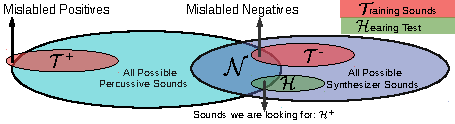
\includegraphics[width=0.95\linewidth]{images/venn_data.pdf}}
    \end{center}
    \caption{ 
    Not to scale (true scales are not measurable and/or subjective).  $\mathcal{N}$ is the set of percussive sounds a synthesizer is capable of making. The inclusion of sounds in this group may vary from person to person. Our positive samples, $\mathcal{T^{+}}$, is a small fraction of a wide variety of percussive sounds that are conceivable. For $\mathcal{T^{-}}$, we can generate any number of random samples. $\mathcal{H}$ is a series of sounds sent to the ear for classification. The ideal ear will detect  $\mathcal{H^{+}}$, the overlap of $\mathcal{H}$ and $\mathcal{N}$, with high precision and recall. 
    }
\label{fig:ven_data}
\end{figure}
\hypref{Decision.1} requires knowledge of what drums \textbf{do not} sound like, or knowledge of an infinitely large set, which cannot be fully represented via examples. An important consideration is that the source of sounds used in training the model (organic drum sounds) will be fundamentally different from the source of unlabeled sounds we wish to categorize (noise from a synthesizer). This issue is reflective of the open set recognition (OSR) problem~\cite{geng2020recent,mundt2019open}. We use figure~\ref{fig:ven_data} to highlight a number of caveats with our training approach: We denote $\mathcal{N}$ as the set of percussive sounds a synthesizer is capable of making. $\mathcal{T^{+}}$, our positive examples, is a set of sound extracted from material drums (see Appendix~\ref{appendix:datasets} for details about our datasets). $\mathcal{T^{-}}$ is a small subset of an infinite set used to represent all noises which the synthesizer is capable of making. Moreover, $\mathcal{T^{-}}$ likely includes sounds in $\mathcal{N}$. During the hearing test, the virtual ear continually receives synthesizer noises for classification. The set of received noises is denoted as $\mathcal{H}$. The performance of the ear is measured by its precision and recall in finding the overlap between $\mathcal{H}$ and $\mathcal{N}$. It is important to ensure that the change in learning domains---particularly with the case of positive examples of percussive sounds---does not interfere with transformation of knowledge from the training of the ear to the hearing test. To maximize the transference of knowledge from one domain to another, we seek to learn from agnostic feature sets that capture fundamental characteristics of the data points.
\subsection{Feature Extraction}
To train our virtual ear, we require generalizable, domain agnostic features. Various works have demonstrated effective reconstruction of signals given their Short-time Fourier Transforms (STFT)~\cite{nawab1983signal,griffin1984signal}. If the STFT of a signal can be used for its reconstruction, perhaps it can be utilized as a source of fundamental features. We defined 3 STFT transformation functions which we believe to capture important, unique attributes of percussive sounds (figure~\ref{fig:stackspectrums}). Our transformations are GPU based, allowing their application in tandem to the training of the classifier or tuning of STFT transformation during hyper-paramter optimization (see Appendix~\ref{appendix:hyperparam}).
\subsection{Ear Types}
\label{classifiers}

Two groups of classifiers are implemented: \emph{two phased ears} (TPEs) and \emph{Mixed Ear Models} (MEMs). TPEs combine different models specializing in~\hypref{Decision.2} or~\hypref{Decision.1} and trained only with our transformation functions. MEMs are a proof of concept attempt at addressing the OSR problem by usage of autoencoded representation of sounds as features. MEMs are trained using highly compressed, automatically encoded representation of sounds and can give simultaneous answers to both questions. Model specifications and extended measurements for TPE and MEMs can be found in Appendix~\ref{appendix:classifier_definitions}. We speculate that the features used to represent sounds plays a much more important role in determining outcomes, particularly when working with relatively small datasets. 

The features used by MEMs are encodings extracted from the latent layer of an autoencoder trained to encode and decode spectrogram representations of sound in MixedDB. To better understand the delineation potential of the encoded features, 64-dimensional latent representation of 20\% of MixedDB and 1000 Noise sounds were projected onto a 2 or 3-dimensional planes using t-SNE. Referring to~\hypref{Decision.1} and~\hypref{Decision.2}, we expect the drum sounds to be clustered together, with the majority of the synthetic noise sounds appearing away from these clusters. The projections confirmed that this is the case ( see Appendix~\ref{appendix:E} for examples of these projections). We are most interested in synthetic noise sounds which appear within or near these clusters. Do these synthetic noise sounds have drum like characteristics?\\ 
To test this, we implemented interactive projection graphs. These graphs allow interactions such as playing the samples(by hovering the cursor on-top) and movement of the scene camera. Manual inspections revealed a noticeable, positive correlation between a synthetic sound's distance and similarity of a synthetic sound to drum clusters.

\section{Pipelines and Surveys}
\label{surveys}
\begin{table}
 \begin{tabular}{|c c c c c c c|} 
 \hline
 Drop Rule & Size & H+H & H+FC & H+CNN & H+E/F & 3 models \\ [0.5ex] 
 \hline
 No Drops & 257 &0.37 & 0.35 & 0.36 & 0.36 & 0.28\\ 
 \hline
 Assigned \enquote{Bad} By Both & 236 & 0.31 & 0.37 & 0.37 & 0.38 & 0.30 \\
 \hline
 Assigned \enquote{Bad} By Either & 180 & 0.47 & 0.50 & 0.48 & 0.48 &  0.34 \\
 \hline
 Assigned \enquote{Bad} or \enquote{Other} By Either & 154 & 0.47 & 0.59 & 0.54 & 0.50 &  0.35 \\
 \hline
\end{tabular}
\caption{\label{kappa_table_TPE}Table of Fleiss' kappa coefficient to measure the degree of agreement between persons (H+H), persons with FC model (H+FC), persons with CNNLSTM model, persons with all models (H+E/F), and between the 3 models. }
\end{table}

 \begin{table}
 \resizebox{\linewidth}{!}{\begin{tabular}{|c c c c|} 
 \hline
 Drop Rule & Size & H+H & H+MEM \\
 \hline
 No Drop & 300 & 0.34 & 0.25\\ 
 \hline
 Assigned Bad By Both & 249 & 0.20 & 0.26 \\
 \hline
 Assigned Bad By Either & 151 & 0.46 &  0.47 \\
 \hline
Assigned \enquote{Bad} or \enquote{Other} By Either  & 120 & 0.62   &  0.59 \\
 \hline
\end{tabular}}
\caption{\label{kappa_table_MEM}Table of Fleiss' kappa coefficient to measure the degree of agreement between persons (H+H) and persons with MEM (H+MEM).}
\end{table}
We built two pipelines and analyzed the results. We the TPE pipeline uses CNNLSTM-DVN for \hypref{Decision.1}, and FC-DVD, CNNLSTM-DVD and E/F for \hypref{Decision.2}. The MEM pipeline uses our best MEM, which simultaneously classifies sounds as drums and categorizes them. 
The TPE pipeline produces samples in the following categories: \enquote{snare}, \enquote{kick}, \enquote{hat}, \enquote{clap} and \enquote{other} (combination of rims, shakers and unusual percussive sounds). The MEM pipeline does not output the \enquote{other} category, yet the option is available to surveyors when categorizing sounds manually.   
We assess the success rate of each pipeline---and by extension, the virtual ears---by manual inspection of sounds categorized as drums. Both authors categorized a subset of the results without knowledge of the assigned labels. Additionally, each responder has the option of labeling samples as \enquote{bad} for samples that they deemed not percussive.  The percentage of sounds labeled as \enquote{bad} by the authors is a measurement of success with regards to \hypref{Decision.1}. We measure success with regards to \hypref{Decision.2}---the reliability of agreement between persons and drum categorization models---via the Fleiss' kappa coefficient \cite{fleiss1971measuring}. The value of 0 or less for this coefficient indicates no agreement beyond random chance, and the values of 1 indicates perfect agreement. We again measure this coefficient after dropping samples that were categorized as \enquote{bad} by one or both authors. We also show measurements after dropping all \enquote{bad} and \enquote{other} samples.
\subsection{Survey Discussion}
\label{survey2_takeaway}
Due to the discrepancy in categorization and output groups, results from the two surveys must be compared with caution. Agree-ability scores for MEM pipeline are often lower, but we reiterate that the MEM survey has two out of six (rather than one out of six in the TPE pipeline) categories which are exclusive to survey responders. Supporting this hypothesis is the notable improvement in agree-ability observed after dropping all \enquote{bad} and \enquote{other} samples. Despite the drawbacks, the MEM pipeline remains competitive while working with a fraction of the features to learn from and simultaneously making both decisions. Suggesting that latent representations of autoencoder networks can be used as general, low-dimensional proxies for representation of complex inputs.

\section{Conclusion and Future Work}
\bibliographystyle{apacite}
\bibliography{CSMC_MUME_LaTeX_Template.bib}


\begin{appendices}
\chapter{Datasets}
\label{appendix:datasets}
Our data sources are a large set of 2 second or shorter drum samples aggregated from personal libraries, free drum kits from the sample-swap project \footnote{https://sampleswap.org/} which we organized into 5 groups, and a large set of drum sounds aggregated from royalty free sources such as musicradar \footnote{https://www.musicradar.com/}. We put together 3 databases of drums using these sources. We also created a database of synthetic noise from 1, 3, and 5 stacked virtual synthesizers. Specifications about our datasets can be found in tables~\ref{db:self},~\ref{db:radar},~\ref{db:sampleswap} and~\ref{db:noise}. We have made our dataset of free-drum sounds available for download. The scripts used to download and process royalty free samples are also made available. Further information about downloading our dataset can be found on the project's github page. 

We prioritize making generalizable tools which can learn from and produce a variety of different sounds. We utilize these databases depending on the task at hand. At times, we merged or purged drum groups to simplify tasks.
\begin{table}[]
\centering
\begin{tabular}[width=\paperwidth]{|l|l|l|l|l|l|l|l|l|l|}
\hline
DB Name & kick & snare & clap & tom\_high & tom\_mid & tom\_low & hihat\_closed &  hihat\_open & rim \\ \hline
MixedDB & 648 & 732 & 118 & 179 & 139 &  188 & 187 & 280 & 105 \\\hline
\end{tabular}
\caption{Database 1: Mixed sources}
\label{db:self}
\end{table}

\begin{table}[]
\centering
\begin{tabular}{|l|l|l|l|l|l|l|l|l|}
\hline
DB Name & kick & snare & clap & tom & clap & hat & rim & shaker  \\ \hline
RadarDB & 1054 & 842   & 353 & 349 &  353 & 1561& 131 & 121 \\ \hline
\end{tabular}
\caption{Database 2: Royalty free sounds sourced from \enquote{Music Radar}}
\label{db:radar}
\end{table}

\begin{table}[]
\centering
\begin{tabular}{|l|l|l|l|l|l|}
\hline
 DB Name & kick & snare & clap & hat & other \\\hline
 FreeDB & 533 & 372 & 230 & 105 & 281 \\ \hline
\end{tabular}
\caption{Database 3: Free sounds sourced from the \enquote{Sample Swap} project. Simplified for our purposes. The version available for download contains more sample groups. The \enquote{other} category contains a variety of percussive sounds.}
\label{db:sampleswap}
\end{table}


\begin{table}[]
\centering
\begin{tabular}{|l|l|l|l|}
\hline
 Synth Noise Type & 1 Stack & 3 Stacks  & 5 Stacks \\ \hline
 Number of Examples & 2000 & 2000 & 2000 \\ \hline
\end{tabular}
\caption{Database of random noise examples from our virtual synthesizers}
\label{db:noise}
\end{table}

%=============
\chapter{Audio Transformation Functions}
\label{appendix:trans_funcitons}
\begin{figure}
\centering
\textbf{Visual Representation of Raw Features}\par\medskip
    \subcaptionbox{Recorded hat sample}{    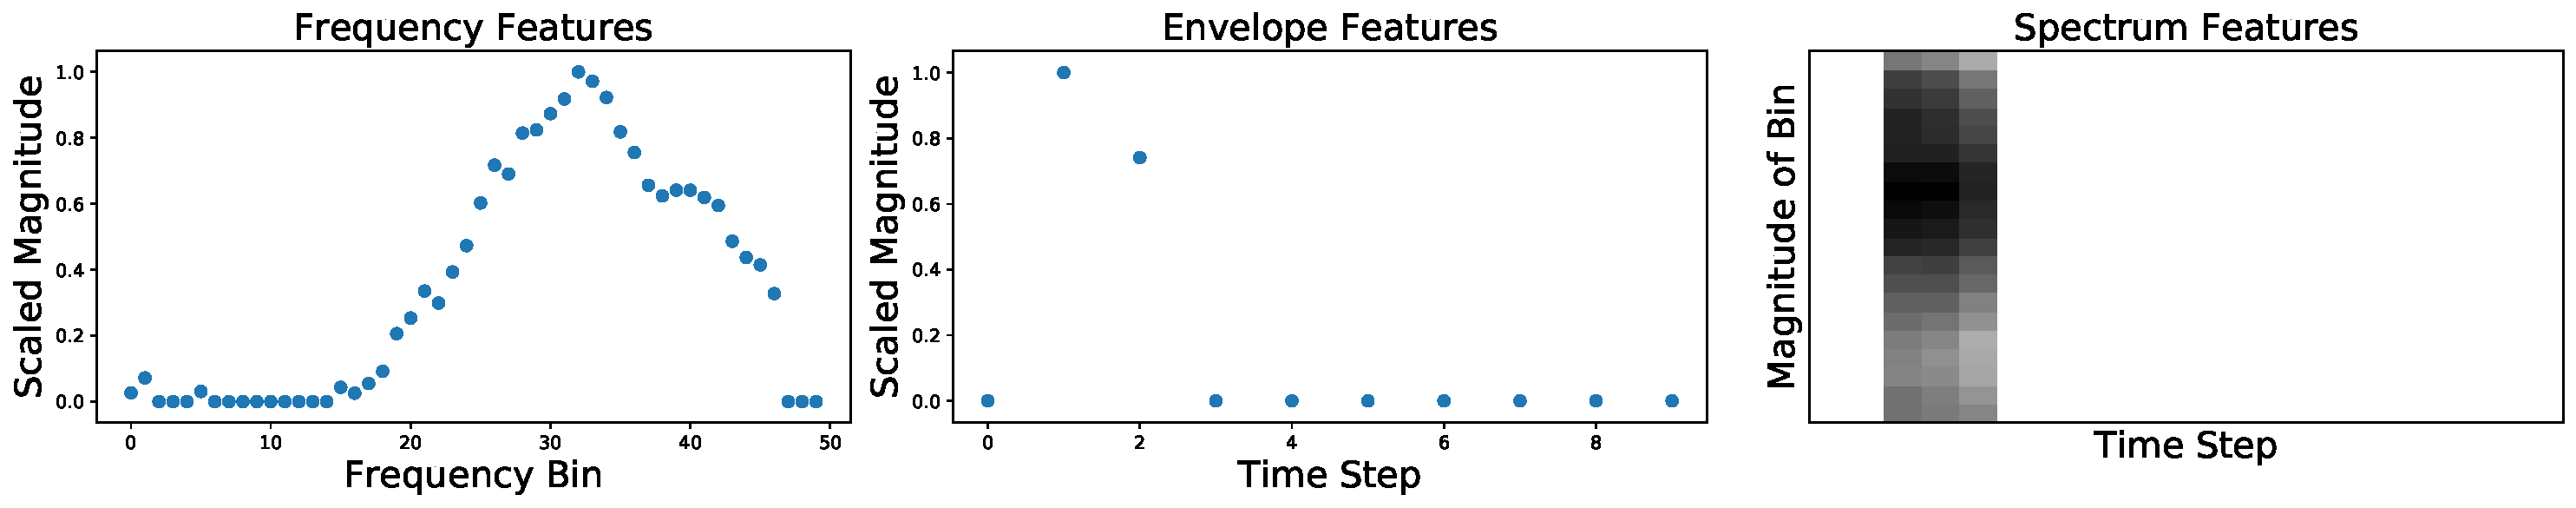
\includegraphics[width=1\columnwidth]{images/ff1.pdf}
    }
    \subcaptionbox{Randomly generated audio with percussive qualities, resembling a tight snare}{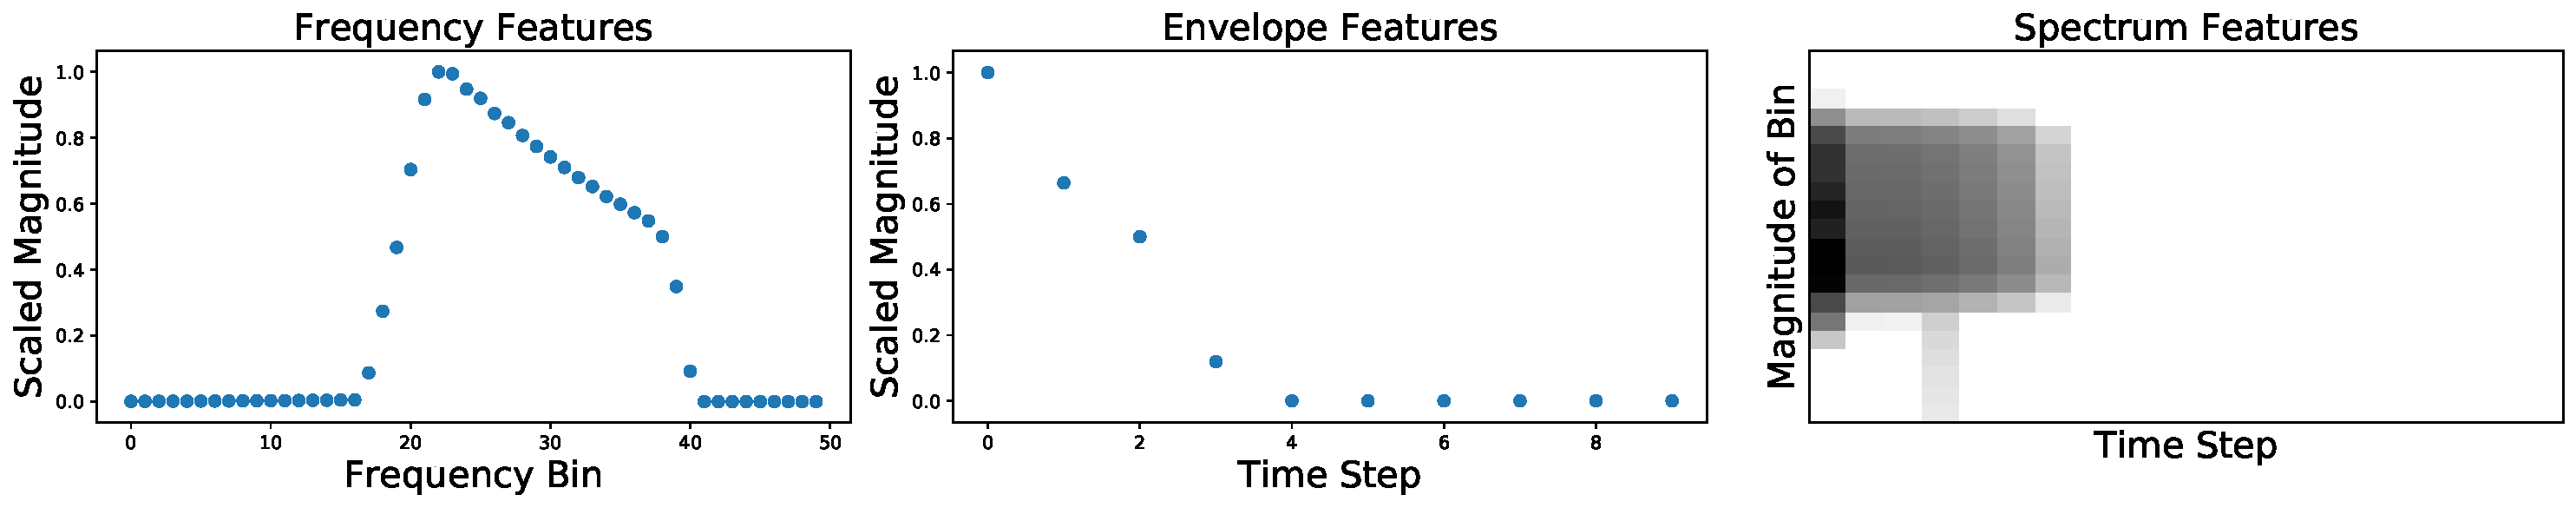
\includegraphics[width=1\columnwidth]{images/ff2.pdf}}
    \subcaptionbox{A randomly generated noise with a percussive envelop but non-percussive frequency features (modulated pitch)}
    { 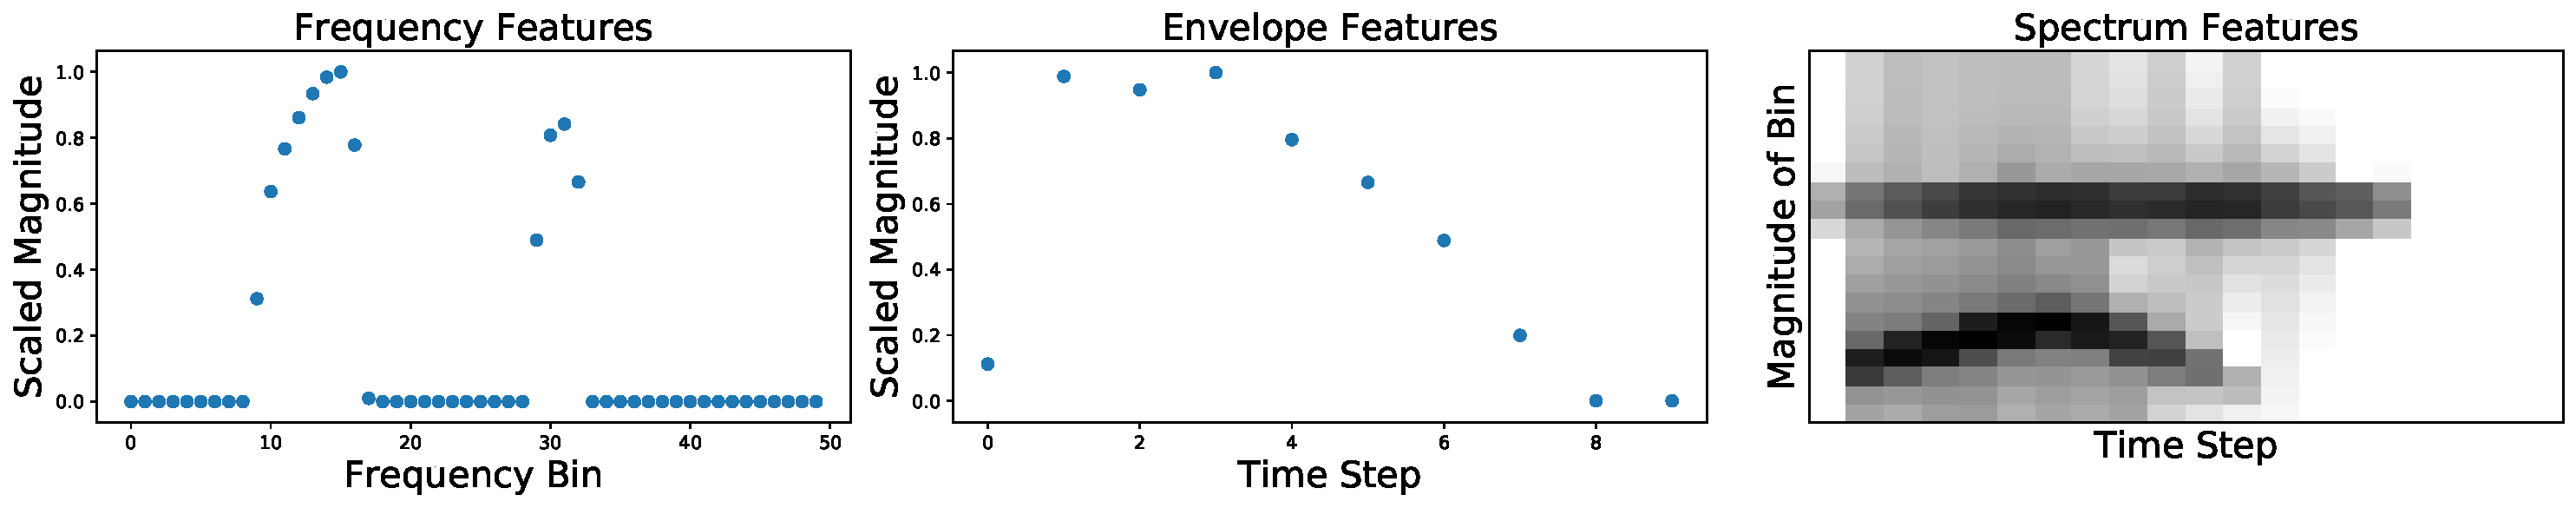
\includegraphics[width=1\columnwidth]{images/ff3.pdf}}
\caption{Graphed representation of features extracted for 3 different samples. Sample $a$ is a recorded hat from our database. sample $b$ is an example of randomly generated noise with percussive qualities that we found suitably similar to a snare sound. Sample $c$ is an example of a randomly generated noise where the spectrum features are necessary for proper classification.}
\label{fig:stackspectrums}
\end{figure}
\begin{enumerate}
\item Envelope Transformation: Represents changes in loudness for the duration of the signal. Using STFT we generate a matrix $M_{i \times j}$ with rows $i$ and columns $j$ corresponding to time steps and frequency bins respectively. Values $v_{i \times j}$ indicating the magnitude of the frequency bin $j$ at each time-step $i$. Information about the envelope of the signal can be extracted by summing the values of $M$ for each time-step (or row $i$), giving us a feature vector that is normalized to the range of 0 to 1. The information contained in this vector is an alternative to Root-Mean-Square measurements of a sliding window over the signal.
\item Frequency Transformation: A static, normalized snap-shot of the the frequencies present within the audio. The calculation of this feature vector is similar to the envelope, but the summation is done along the frequency axis. Another important distinction is that since capturing an adequate frequency resolution is important for this transformation, we utilized shorter hop-sizes and wider windows. A Mel Scale transformation was also applied in hopes that the captured features better represent human perception of frequencies. 
\item Spectrum Transformation: This function is simply a Mel Scaled STFT with its values normalized from 0-1. Spectrograms contain more information about the original signal but their analysis requires more complex computational methods.
\end{enumerate}

%================
\chapter{Virtual Ear Classifier Definitions}
\label{appendix:classifier_definitions}
\section{Two Phased models}
Using the described features, we trained several neural network models for Phase 1 and 2 in the Pytorch environment. The task of Phase 1 is to separate drums from not-drums (DrumVsNotDrum, or DVN). The task of Phase 2 is to categorize drums and percussion (DrumVsDrum, or DVD). We kept our feature space small, making it viable for feature selection and model design to be done on a trial and error basis. For all models, accuracy is calculated by prediction of all test dataset labels and the loss function and optimizer are Categorical-CrossEntropy and Adam respectively. Training continues until no reduction in loss and accuracy is observed in 10 epochs.  All activation functions are PReLU:
\begin {enumerate}
\item FC-DVN: Fully connected network trained on Envelope features, reaching 97\% accuracy on our test data for Phase 1. With size of 10x5x10.
\item CNNLSTM-DVN: A combination of CNN and LSTM models, where the CNN model extracts higher level features that are fed temporally to an LSTM cell. This model is trained on spectrum data and reaches 98\% accuracy on our test set. Its structure is the combination of a CNN with 2 output channels and kernel size $(7,3)$; Followed by an LSTM model of hidden size 800 and a fully connected layer of size 20x2.
\item E/F-DVD: A fully connected model trained on a concatenation of envelope and frequency features. Reaching 80\% accuracy for 6-way drum categorization in Phase 2. Size of 50x10x2x6.
\item CNN-DVD: A CNN model trained on Spectrum features. Reaching 82\% accuracy in a 6-way drum categorization in Phase 2. A combination of a CNN model with output channel size of 4, kernel of size of 5, another CNN model with output channel size of 8 and kernel of size 3. Followed by a fully connected network of shape 100x20x6.
\item FC-DVD: Fully connected 3 layer neural net with 78\% accuracy for 6-way drum categorization in Phase 2. Size of 400x200x50.
\end{enumerate}
Unlike EE models, parameters are hand-picked and un-tuned. Higher accuracy rates in these models do not necessarily translate to higher agreeableness with surveyors. Since the positive sounds in the hearing test are sourced from a synthesizer, model accuracy on test data alone cannot be relied upon when the domain of sounds 
being categorized is switched.

%========

%==============
\chapter{AutoEncoder Structures and Hyper-Parameter Optimization}
\label{appendix:hyperparam}
% could do multi-objective pareto front stuff too
Within the context of machine learning, a model's \emph{hyper-parameters} are fixed parameters which are set before the training begins (e.g number of layers, size of layers, loss function) and are not learned during the minimization procedure~\cite{bengio2000gradient}. To assist us with the construction of our model, we defined a number of possible choices for the architecture of our model and audio-transformers and used hyper-parameter optimization to extract promising sets of values~\ref{table:hyper_params}. 

The list of possible choices for the selected hyper-parameters can be found in table~\ref{table:hyper_params}. We included not only model parameters but also spectrogram transformation parameters within this search space, as GPU accelerated FFT calculations allows ad hoc audio transformations to take place parallel to the training process. We implemented 3 base models which are affected by these hyper-parameters. The \enquote{Model Type} parameter dictates whether CNN or fully connected models are selected; If a \enquote{fully connected} model is selected, the \enquote{hidden layers} parameter selects between the two implementations. The specifications for these models can be found in tables~\ref{table:FC1_AUTOENCODER},~\ref{table:FC2_AUTOENCODER} and~\ref{table:CNNAUTOENCODER}.

Using the optuna optimization tools \cite{akiba2019optuna}, we conducted 500 search trials. The trial's success is measured in their final loss value, calculated by applying the model to test data-set. Each trials consisted of 20 epoch of training using a selected set of hyper-parameters. An additional 100 trials with 40 epochs of training were conducted following the initial 500 to test the effect of longer epochs. Each trial's intermediate results (loss at every n epoch,s where $0<n<20$) were reported to a multi-armed bandit based pruner for early stoppage of unpromising trials~\cite{li2017hyperband}. We employed a tree-structured parzen estimator for better navigation of the search space~\cite{bergstra2011algorithms,akiba2019optuna} but found short reversions to a random sampling coupled with a decrease in the frequency of pruning helpful in exiting local minima. \\
\begin{table}[htbp]

\begin{tabular}{|p{28mm}|p{50mm}|p{21mm}|p{21mm}|}
\hline
Hyper-Param. & Description  & Values & Distribution\\ \hline
Model Type      &   Affects encoder's first hidden layer & CNN,FC & Categorical \\  \hline
Optimizer       & Updates network's weights based on loss & Adam,SGD & Categorical  \\  \hline
Hidden Layers   & Extra hidden layer for the Encoder & True,False & Categorical \\  \hline
Time Steps & Temporal granularity of the spectrogram. Affects FFT windowing. & 10,20 & Categorical  \\ \hline
Learning Rate   &    Optimizer's learning rate  & $1^{-4}$ ... $1^{-1}$ & Uniform      \\ \hline
Frequency Bins & Number of spectrogram frequency bins & 10, 30,60 & Categorical \\ \hline

Regularization  &  L2 regularization parameter. Penalizes large weights to prevent overfitting & 1^{-6}~...~1^{-1} & Uniform\\ \hline
Latent Size & Size of bottle neck layer or number encoded features & 8,16,64 & Categorical              \\ \hline
Dropout Rate & Random zeroing of activations between layers to prevent over-fitting & 0,0.5,0.1 & Categorical\\  \hline
\end{tabular}
\caption{The Hyper-Paramter space in which the optimization was conducted.}
\label{table:hyper_params}
\end{table}
\begin{table}
\begin{tabular}{|p{3cm}|p{3cm}|p{3cm}|p{3cm}|}
\hline
Layer-\# & Out Shape & Param Num & Details  \\ \hline
Conv2d-1 & [-1, 8, 30, 20] &   208 & Encoder's input \newline
Num. Channels:8\newline
kernel:5x5\newline                  
stride:1\newline    
padding:2 \\ \hline
ReLU-2 & [-1, 8, 30, 20] &   0 & \\  \hline
MaxPool2d-3 & [-1, 8, 15, 10] & 0 &  kernel:5x5 \newline
stride:2 \\ \hline
Dropout-4 & [-1, 8, 15, 10] & 0 &  \\ \hline
Linear-5 & [-1, 8] & 9,608 & Encoder's output \\ \hline
Linear-6 & [-1, 256] & 2,304 & Decoder's Input \\ \hline
Dropout-7 & [-1, 256] & 0 &  \\ \hline
Linear-8 & [-1, 600 ] &  154,200& Decoder's output\\ \hline
\end{tabular}
\caption{CNN model design with latent size of 8. 30 and 20 are the assumed frequency bins and step size. Total number of parameters is 166,320. }
\label{table:CNNAUTOENCODER}
\end{table}

\begin{table}
\begin{tabular}{|p{3cm}|p{3cm}|p{3cm}|p{3cm}|}
\hline
Layer-\# & Out Shape & Param Num & Details  \\ \hline
Linear-1 & [-1, 128]  & 76,928 & Encoder's input \\ \hline
Dropout-2 & [-1, 128] & 0 &  \\ \hline
Linear-3 & [-1, 8] & 9,608 & Encoder's output \\ \hline
Linear-4 & [-1, 128] & 2,304 & Decoder's Input \\ \hline
Dropout-5 & [-1, 128]  & 0 &  \\ \hline
Linear-6  & [-1, 600 ] &  77,400 &Decoder's output\\ \hline
\end{tabular}
\caption{Fully connected model with only 1 hidden dimension for encoder and decoder. Designed assumes latent size of 8. 30 and 20 are the assumed frequency-bins and step-size values. Total number of parameters is 156,512.}
\label{table:FC1_AUTOENCODER}
\end{table}

\begin{table}

\begin{tabular}{|p{3cm}|p{3cm}|p{3cm}|p{3cm}|}
\hline
Layer-\# & Out Shape & Param Num & Details  \\ \hline
Linear-1 & [-1, 128]  & 76,928 & Encoder's input \\ \hline
Dropout-2 & [-1, 128] & 0 &  \\ \hline
Linear-3 & [-1, 32]  & 4,128 & \\ \hline
Dropout-4 & [-1, 128] & 0 &  \\ \hline
Linear-5 & [-1, 8] & 9,608 & Encoder's output \\ \hline
Linear-4 & [-1, 32] & 2,304 & Decoder's Input \\ \hline
Dropout-5 & [-1, 32]  & 0 &  \\ \hline
Linear-4 & [-1, 128] & 2,304 & \\ \hline
Dropout-5 & [-1, 128]  & 0 &  \\ \hline
Linear-6  & [-1, 600 ] &  77,400 &Decoder's output\\ \hline
\end{tabular}
\caption{Fully connected model with 2 hidden dimensions for encoder and decoder. Designed assumes latent size of 8. 30 and 20 are the assumed frequency-bins and step-size values. Total number of parameters is 163,232.}
\label{table:FC2_AUTOENCODER}
\end{table}

\begin{figure}[htbp]
\centering
\textbf{Tracing the Best Loss Values}
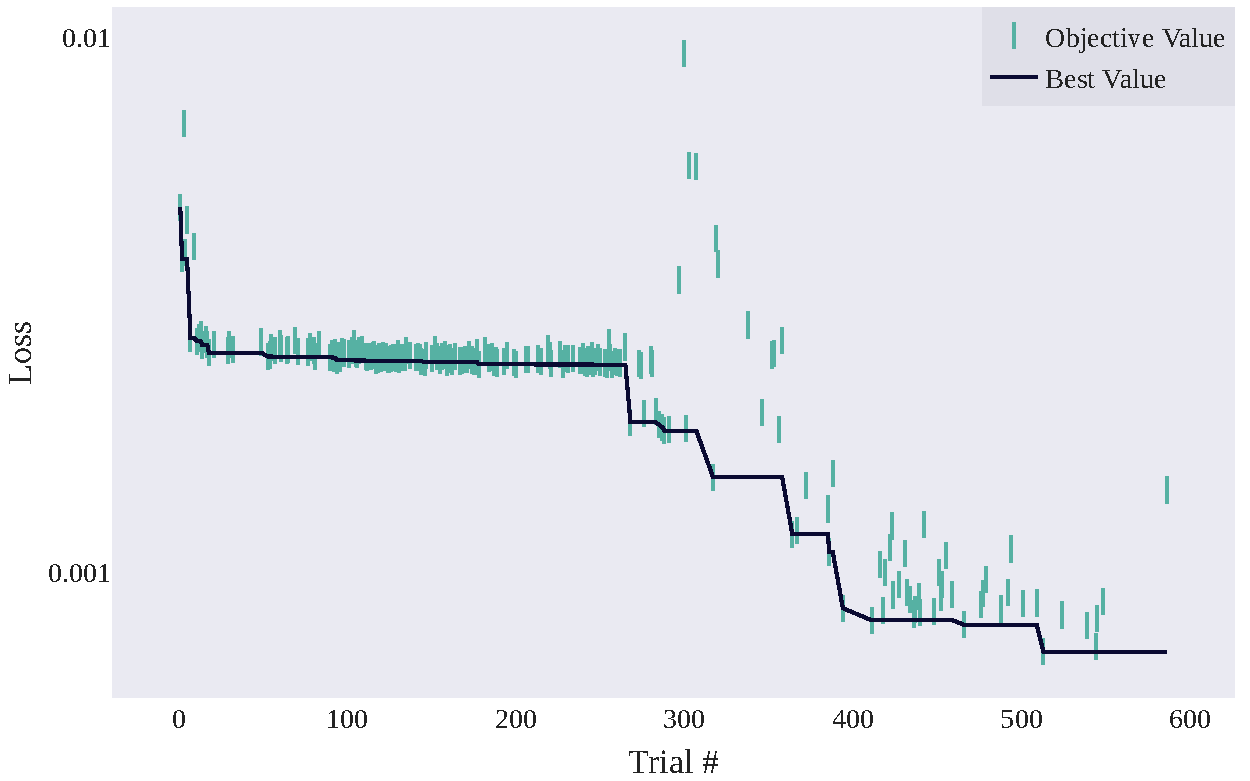
\includegraphics[width=12cm,height=7cm]{images/Optimization_History.pdf}
\caption{Best loss values found during hyper-parameter optimization. The effect of a switch to random sampling and an increase of the pruning threshold can be observed during trials 270 and 310.}
\label{chap3:bestvalues}
\end{figure}

\begin{figure}
\begin{center}
    \textbf{Hyper-Parameters' Loss Correlation}
    \makebox[\textwidth]{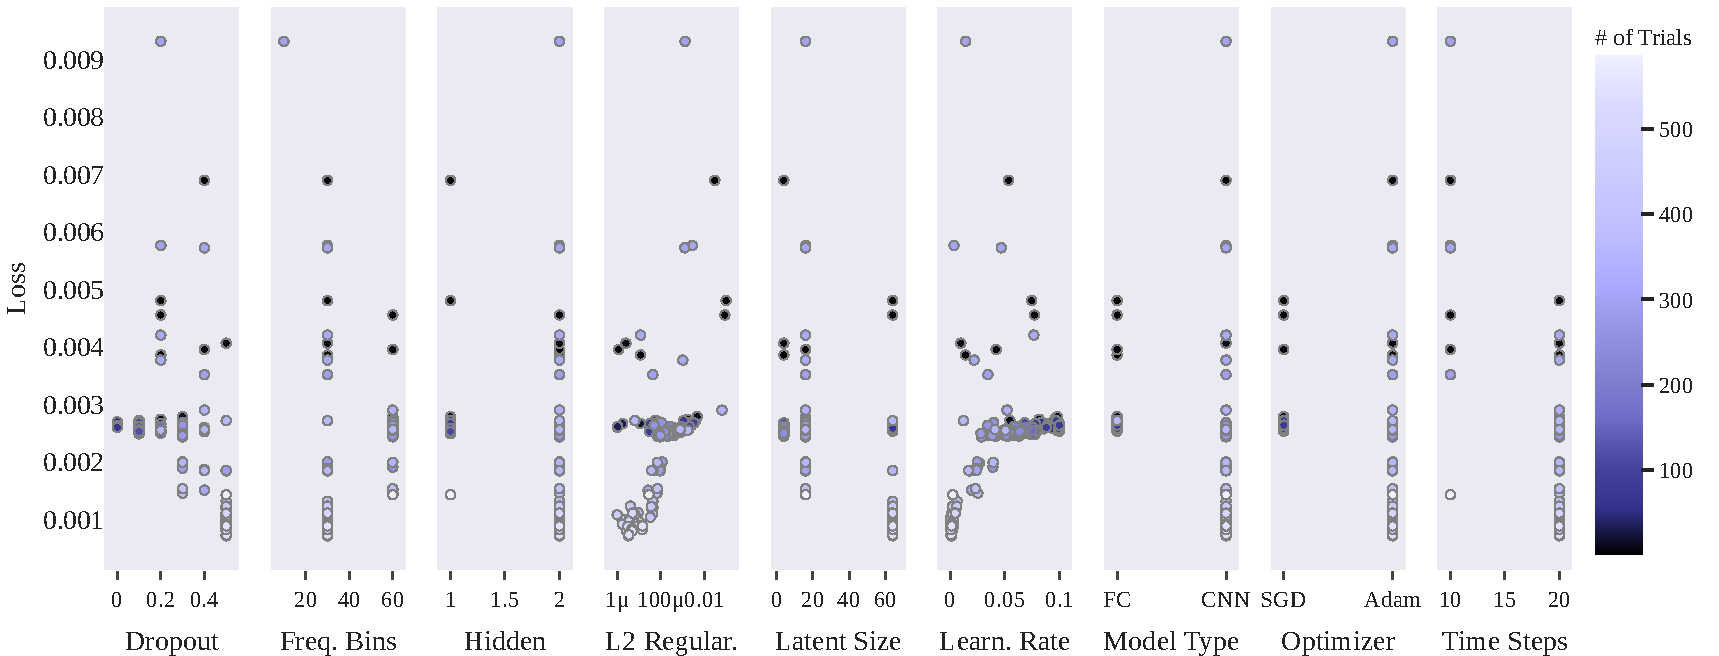
\includegraphics[width=0.95\paperwidth]{images/slice_plot.pdf}}
      \caption{Sliced plot depicting the correlation between hyper-parameters and loss values. The color-scale shows the number of times each parameters has been used in a trial. Our sampling algorithm aims to utilize spaces with higher potential more often. }
    \label{fig:slicegraph}
    \end{center}

\end{figure}

\begin{table}[htbp!]
\centering
\begin{tabular}{|p{6cm}|p{6cm}|}
\hline
Hyper-Param. & Value  \\ \hline
Model Type      &  CNN  \\ \hline
Optimizer       & Adam  \\ \hline
Hidden Layers   & Not Applicable  \\\hline
Learning Rate   &  0.001145\\ \hline
Frequency Bins & 30 \\ \hline
Time Steps & 20 \\ \hline
Latent Size & 64 \\ \hline
Regularization & 3.25^{-6}\\ \hline
Dropout Rate & 0.5 \\ \hline
\end{tabular}
\caption{Top performing hyper-parameter set}
\label{table:best_params}
\end{table}


%==============
\chapter{Embedded Feature Visualization}
Live demos provided in project source code.
\label{appendix:E}
\begin{figure}[]
\centering
\textbf{2 Dimensional Projection of Latent Variables}\par\medskip
 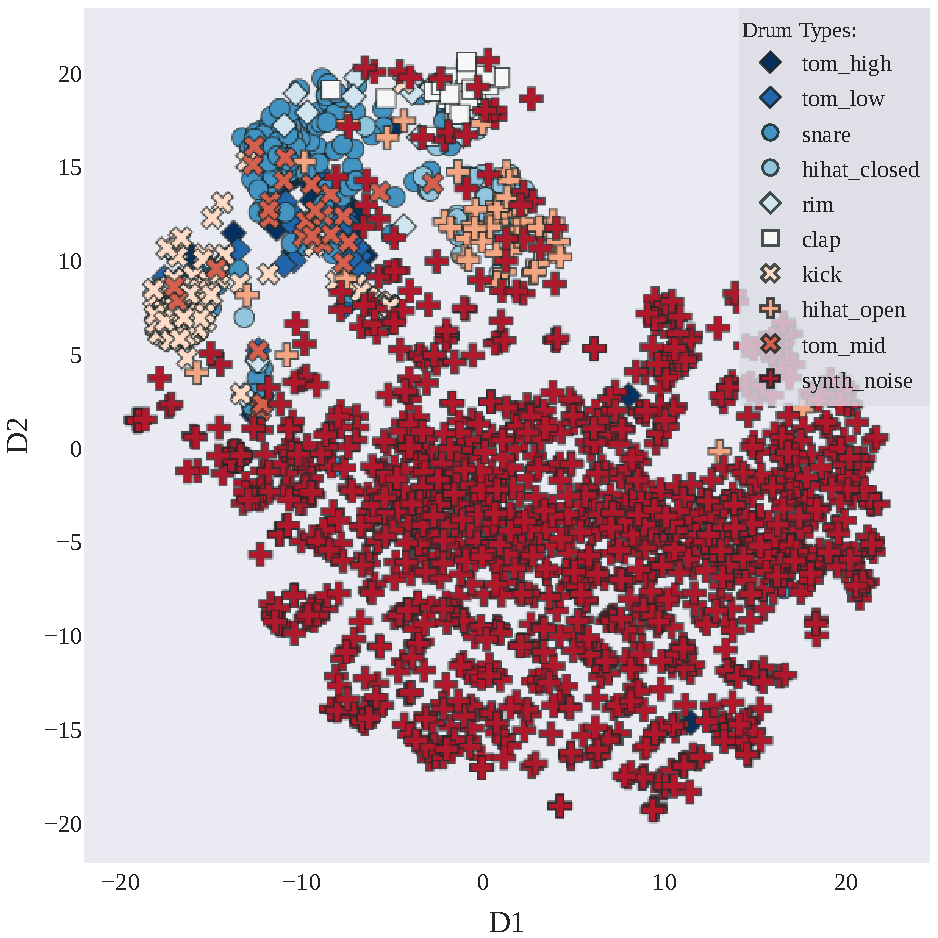
\includegraphics[width=0.90\linewidth]{images/t-SNE_2d.pdf}
\caption{Projection of an embedding model's low dimensional encoding on to a 2D plane. We implemented interactions for these graphs for manual inspection of samples. }
\label{fig:2d_tsne}
\end{figure}

\begin{figure}[]
\centering
\textbf{3D t-SNE Projection}\par\medskip
\mbox{\subfloat[]{\label{subfig:1} \fbox{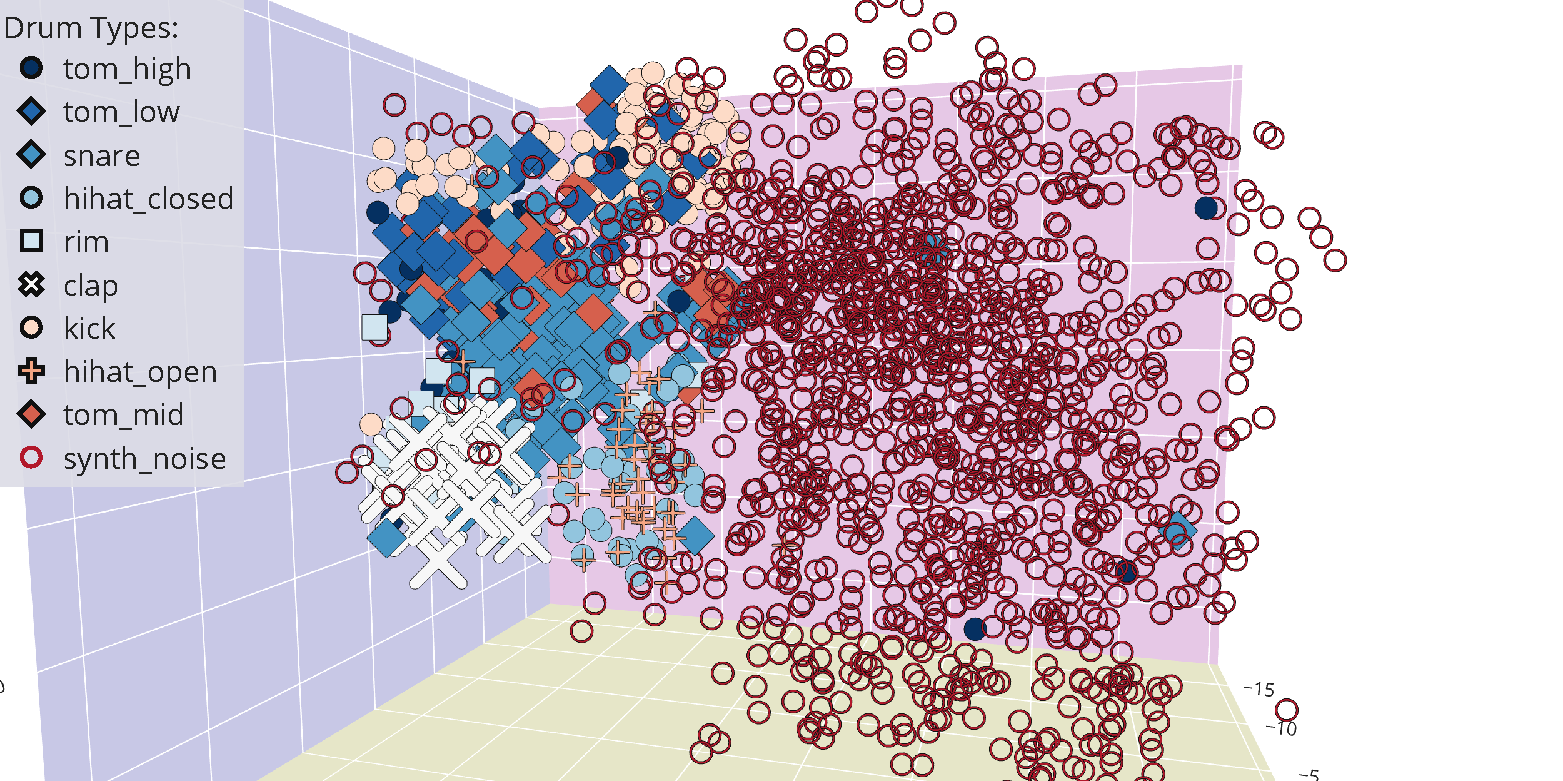
\includegraphics[width=12cm,height=6.8cm]{images/3d_t-SNE_symdrum_type_cam0.pdf}}}}

\mbox{\subfloat[]{\label{subfig:2} \fbox{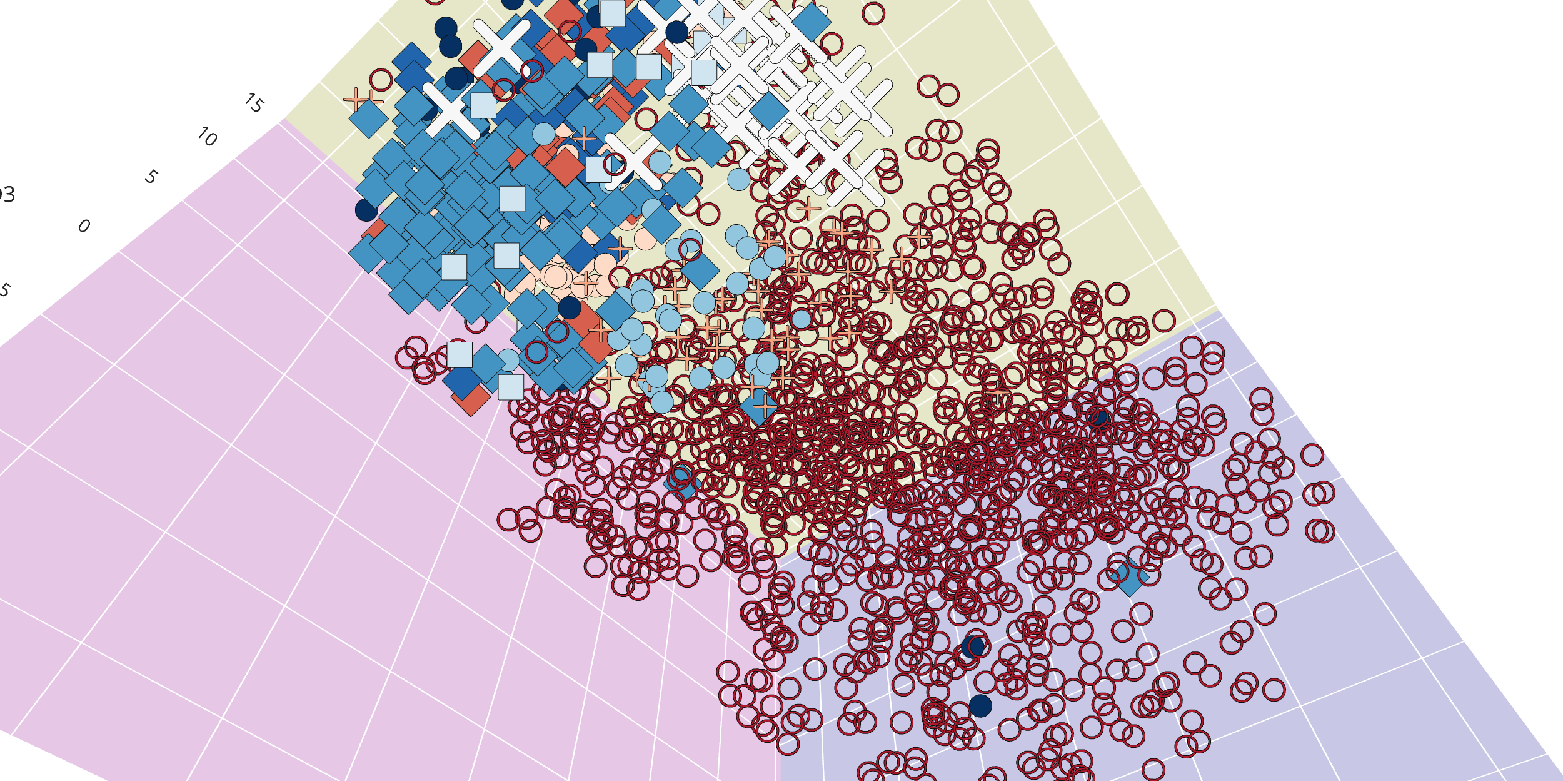
\includegraphics[width=12cm,height=6.8cm]{images/3d_t-SNE_symdrum_type_cam3.pdf}}}}

\fbox{\mbox{\subfloat[]{\label{subfig:2} 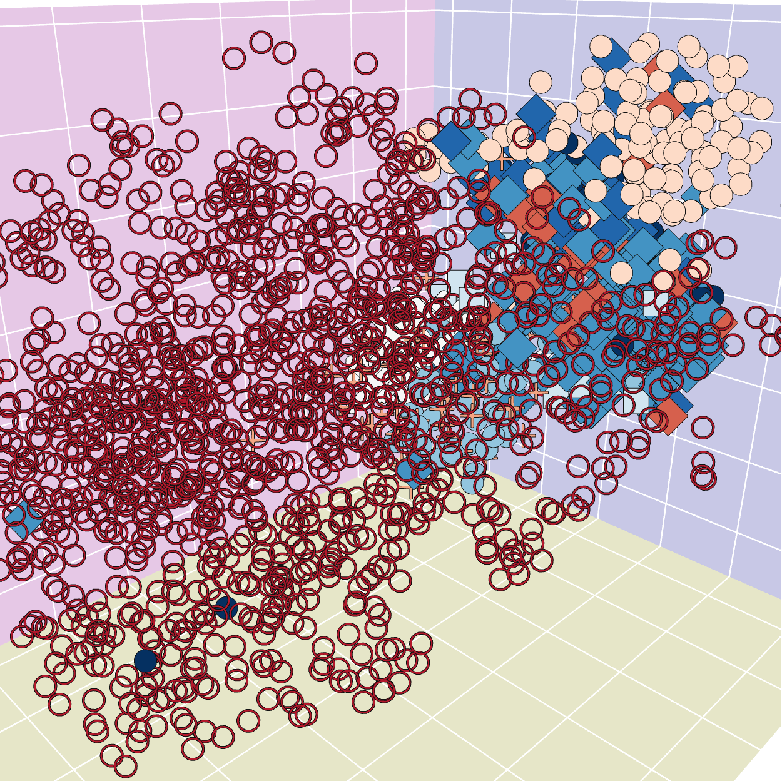
\includegraphics[width=6cm,height=6cm]{images/3d_t-SNE_symdrum_type_cam1.pdf}}}
\mbox{\subfloat[]{\label{subfig:2} 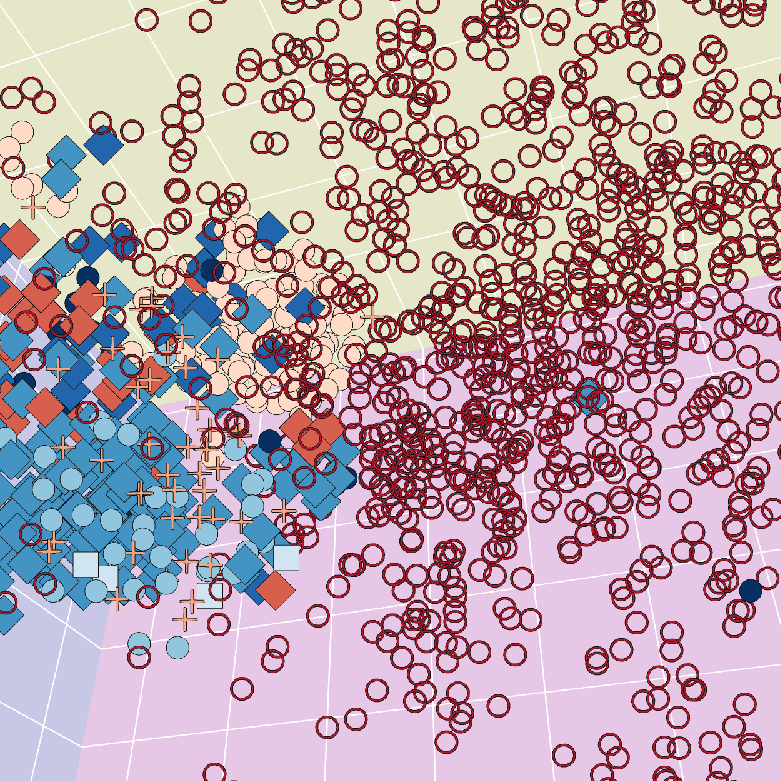
\includegraphics[width=6cm,height=6cm]{images/3d_t-SNE_symdrum_type_cam2.pdf}}}}
\caption{3D projections of the data used for Figure~\ref{fig:2d_tsne}. Interactive demos are also implemented for 3D projections.}
\label{fig:3d_tsne}
\end{figure}


%==============
\chapter{Survey Details}
\label{appendix:surveys}
\subsubsection{TPE Survey of 257 Samples:}
\begin{itemize}
    \item With 6 categorization groups, responders had the same categorization in 47\% of cases.
    \item The agreement between the responders and AVG was 44\% and 47\%.
    \item Of 257 samples, the responders agreed with FC, CNNLSTM and E/F respectively in 78, 76, and 46 of cases. The loss of spectrum data is likely the cause of E/F model's noticeably worse performance. 
    \item The survey brings into question the reliability of our phase 1 model, as 30\% of the generated samples were deemed not percussive by at least 1 reviewer and 8\% by both reviewers
    \item The task of categorizing synthetic drums is difficult. Survey shows that the scale of agreement within persons as well as between persons and various model combinations is moderate at best, even after removal of \enquote{bad} samples.  While the same models can easily achieve 98+ percent accuracy when tested on sounds from physical drum samples. 
    \item While there is much room for improvement, our pipelines can generate and categorize drums and percussive sounds with a promising degree of success. 
\end{itemize}

\begin{figure}[h!]
    \begin{center}
    \textbf{Category Assignment Frequency For TPE Survey}
    \makebox[\textwidth]{
    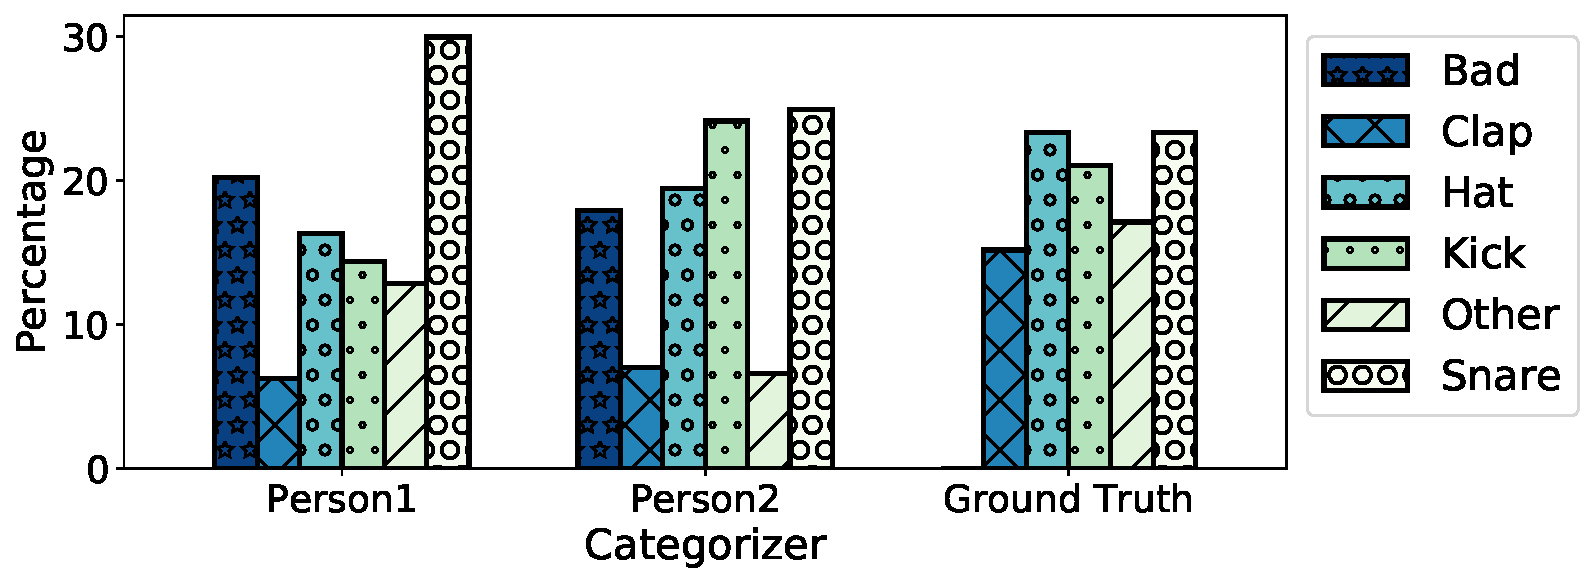
\includegraphics[width=1.1\linewidth]{images/cat_2p.pdf}}
    \end{center}
    \caption{Frequency of assigned labels by persons vs the true number of labels}
\label{fig:freq-survey-2p}
\end{figure}

\subsubsection{MEM Survey of 300 Samples:}

\begin{figure}[htpb]
    \begin{center}
    \textbf{Category Assignment Frequency For MEM Survey}
    \makebox[\textwidth]{
    \includegraphics[width=1.1\linewidth]{images/cat_MME.pdf}}
    \end{center}
    \caption{Frequency of assigned labels by persons vs the true number of labels}
\label{fig:freq-survey-2p}
\end{figure} 


\end{appendices}
\end{document}
